\documentclass[aspectratio=169]{beamer}
\usepackage[english]{babel}
\usepackage[utf8]{inputenc}

% AMSLaTeX packages
\usepackage{amsthm}
\usepackage{amsmath}
\usepackage{amsfonts}
\usepackage[algoruled]{algorithm2e}

\usetheme{default}
\useoutertheme{default}
% we want to use images
\usepackage{graphicx}
\usepackage{movie15}
\usepackage{hyperref}

% table relates packages
\usepackage{booktabs}
\usepackage{multirow}
% pick a font
\usepackage{palatino}           
% \usepackage{times}
\usepackage{tikz}
\usetikzlibrary[positioning,arrows,decorations.pathmorphing,backgrounds,fit,calc]
% \AtBeginSection[]  % "Beamer, do the following at the start of every section"
% {
%   \begin{frame}<beamer> 
%     \frametitle{Outline} % make a frame titled "Outline"
%     \tableofcontents[currentsection]  % show TOC and highlight current section
%   \end{frame}                    
% }

% \AtBeginSubsection[]
% {
%   \begin{frame}
%     \frametitle{Outline}
%     \tableofcontents[currentsection,currentsubsection]
%   \end{frame}
% }

\AtBeginSection[]
{
   \begin{frame}
       \frametitle{Outline}
       \tableofcontents[currentsection]
   \end{frame}
}

\newcommand{\ebox}[1][1em]{\framebox[#1]{\phantom{M}}}

\setlength\arraycolsep{1.4pt}% some length

%gets rid of navigation symbols
\setbeamertemplate{navigation symbols}{}

%gets rid of bottom navigation bars
\setbeamertemplate{footline}[page number]{}
\setbeamertemplate{headline}{}


\usebackgroundtemplate{
\includegraphics[width=\paperwidth]{../../templates/NormalANLBlue}}
\title{A framework for fully autonomous design of materials via multiobjective optimization and active learning:
challenges and next steps}
\author{Tyler Chang$^{\star a}$,
Jakob Elias$^b$,
Stefan Wild$^{a\rightarrow c}$,
Santanu Chaudhuri$^{b,d}$ \& Joe Libera$^b$}
\institute{$^a$Mathematics and Computer Science Division, Argonne National Laboratory\\
$^b$Applied Materials Division, Argonne National Laboratory\\
$^c$Applied Mathematics and Computational Research Division, Lawrence Berkeley National Laboratory\\
$^d$Department of Civil, Materials, and Environmental Engineering, University of Illinois Chicago}
\date{ICLR 2023 Workshop on ML4Materials (May 2023)}
\begin{document}

\setbeamertemplate{footline}{}
{
%\usebackgroundtemplate{
\includegraphics[width=\paperwidth]{../../templates/TitleANLBlue}}
\frame{\titlepage}
}

\setbeamertemplate{footline}[page number]{}

%%%%%%%%%%%%%%%%%%%%%%%%%%%%%%%%%%%%%%%%%%%%%%%%%%%%%%%%%%%%%%%%%%%%%%%%%%%%%%
\begin{frame}
\frametitle{Big Picture}
%%%%%%%%%%%%%%%%%%%%%%%%%%%%%%%%%%%%%%%%%%%%%%%%%%%%%%%%%%%%%%%%%%%%%%%%%%%%%%
  The Argonne Material Engineering Research Facility (MERF):
  \begin{center}
  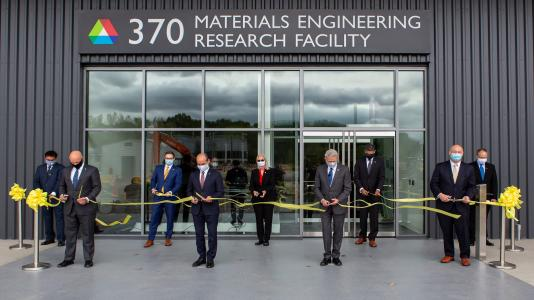
\includegraphics[width=0.45\textwidth]{../../img/probs/merf-ribbon-cutting.jpg}
  \end{center}

  \bigskip

  Accelerate experimentation $\rightarrow$ production pipeline with ML:
  \begin{center}
  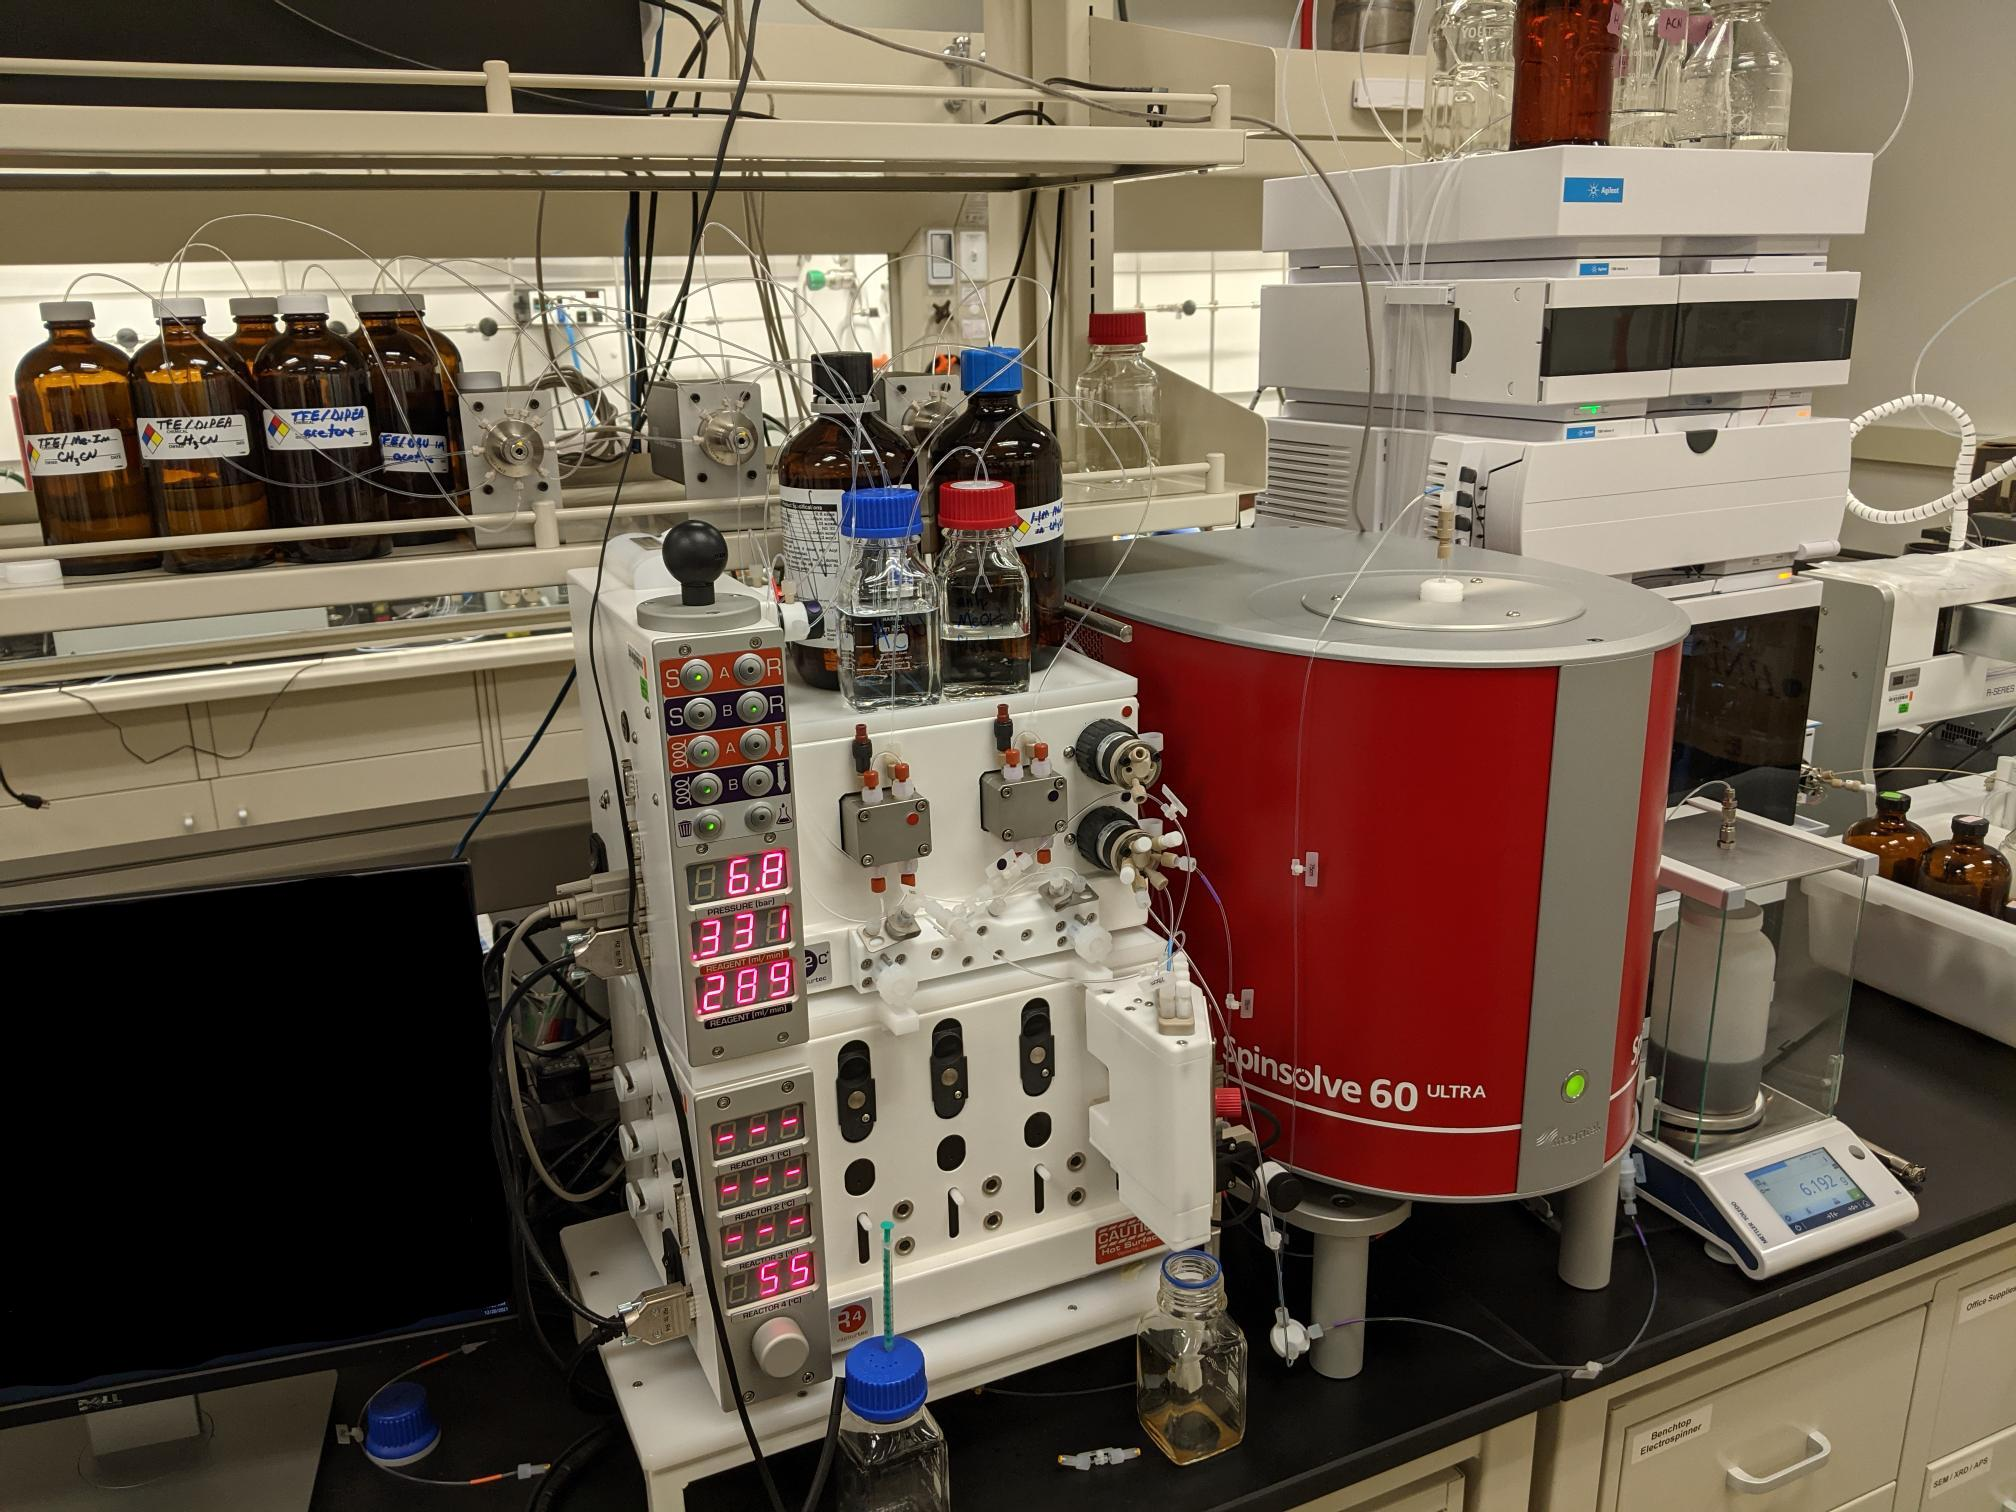
\includegraphics[width=0.2\textwidth]{../../img/probs/cfr-nmr-setup.jpg} $\leftarrow$
  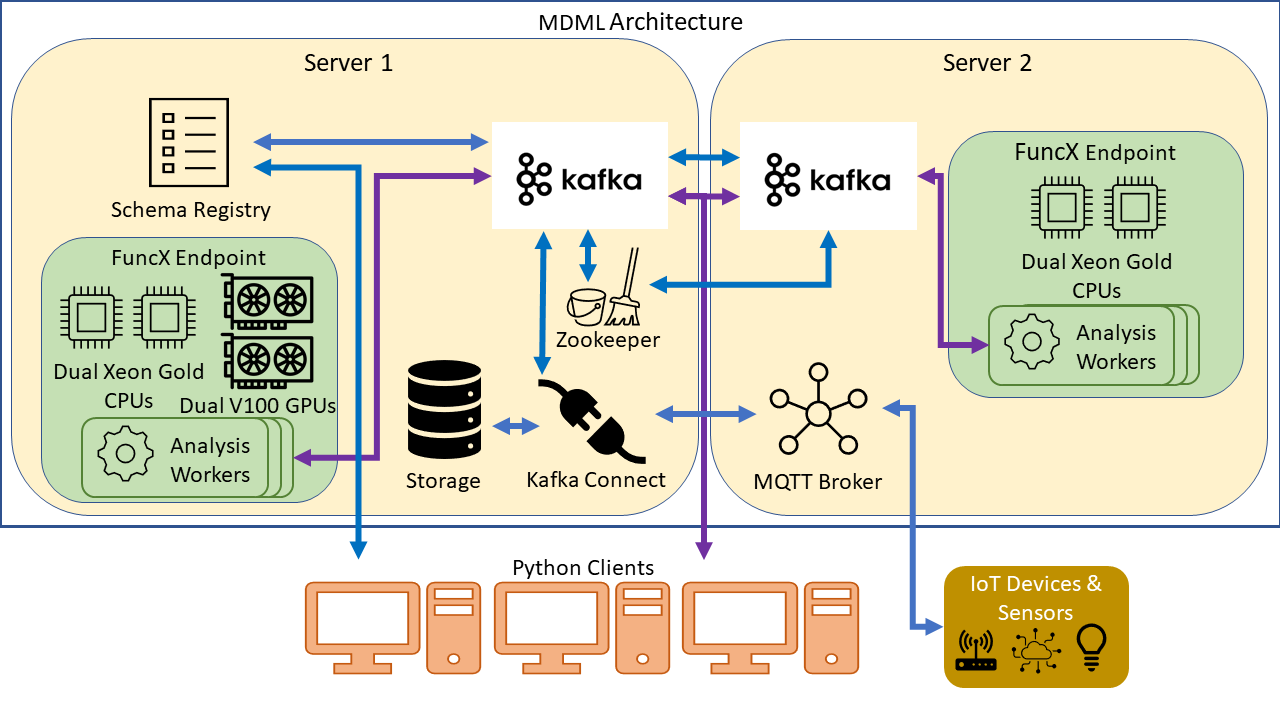
\includegraphics[width=0.3\textwidth]{../../img/moo_new/MDML_arch_v2.png} $\rightarrow$
  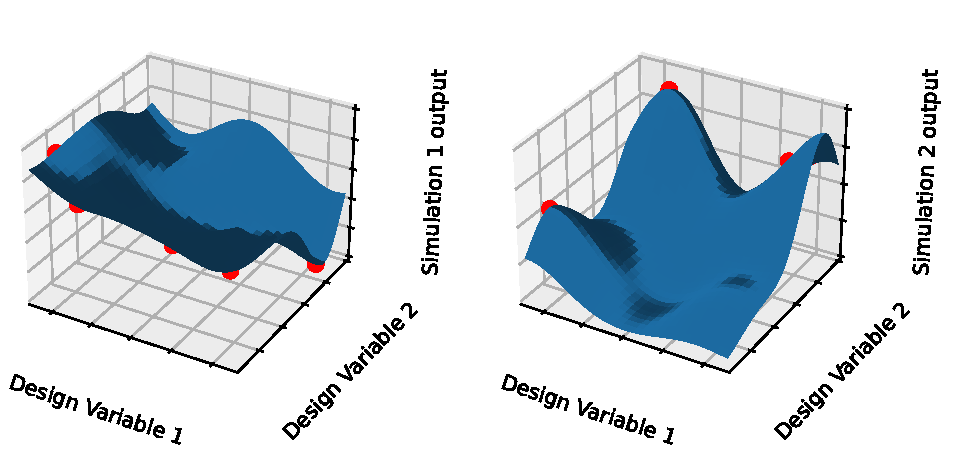
\includegraphics[width=0.3\textwidth]{../../img/moo_old/surrogate-models.pdf}
  \end{center}
\end{frame}

%%%%%%%%%%%%%%%%%%%%%%%%%%%%%%%%%%%%%%%%%%%%%%%%%%%%%%%%%%%%%%%%%%%%%%%%%%%%%%
\begin{frame}
\frametitle{Our (Big) Goals}
%%%%%%%%%%%%%%%%%%%%%%%%%%%%%%%%%%%%%%%%%%%%%%%%%%%%%%%%%%%%%%%%%%%%%%%%%%%%%%
  \begin{itemize}
  \item Design a software framework for {\sl self-driving labs}
  \item Accelerate discovery via intelligent experimentation
  \item Democratize lab-work by building open-source tools
  \end{itemize}
\end{frame}

%%%%%%%%%%%%%%%%%%%%%%%%%%%%%%%%%%%%%%%%%%%%%%%%%%%%%%%%%%%%%%%%%%%%%%%%%%%%%%
\begin{frame}
\frametitle{Streaming data from multiple sources}
%%%%%%%%%%%%%%%%%%%%%%%%%%%%%%%%%%%%%%%%%%%%%%%%%%%%%%%%%%%%%%%%%%%%%%%%%%%%%%
  \begin{itemize}
  \item How to collect and analyze data?
  \item MDML is a platform for streaming, analyzing, and
  logging experiment and simulation data (used at the MERF)
  \end{itemize}
  \begin{center}
  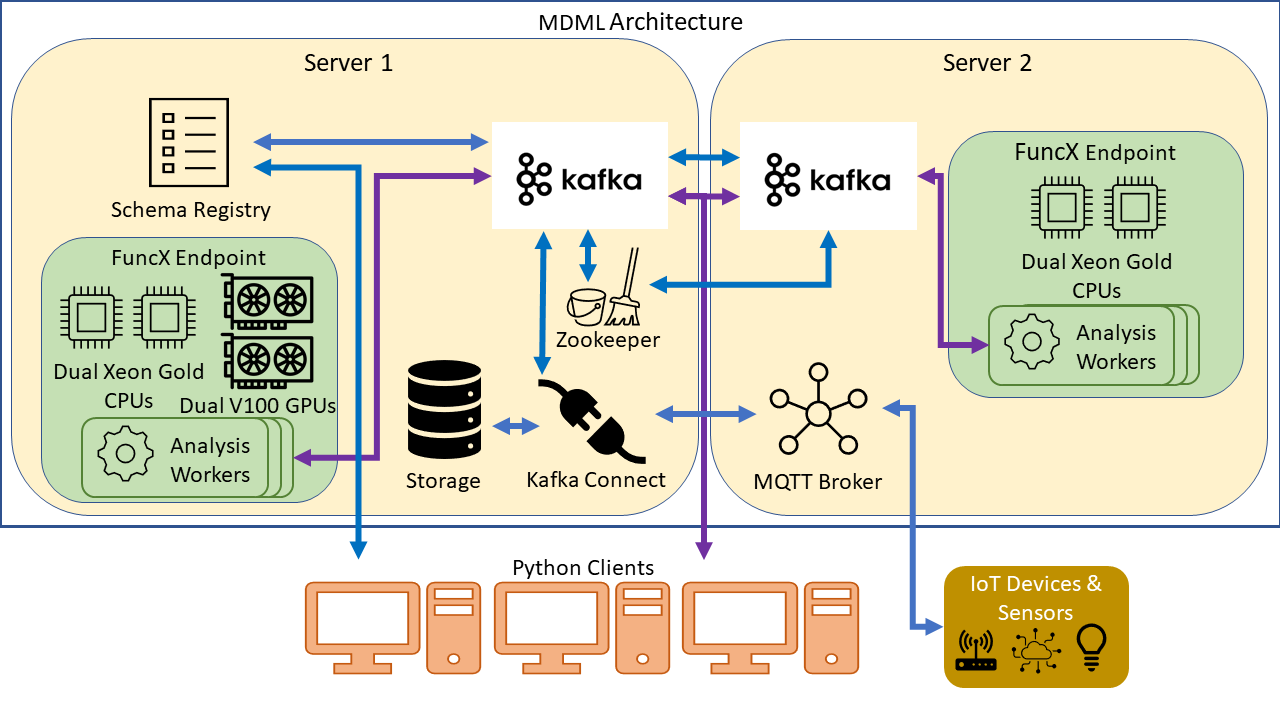
\includegraphics[width=0.85\textwidth]{../../img/moo_new/MDML_arch_v2.png}
  \end{center}
\end{frame}

%%%%%%%%%%%%%%%%%%%%%%%%%%%%%%%%%%%%%%%%%%%%%%%%%%%%%%%%%%%%%%%%%%%%%%%%%%%%%%
\begin{frame}
\frametitle{Model-based optimization}
%%%%%%%%%%%%%%%%%%%%%%%%%%%%%%%%%%%%%%%%%%%%%%%%%%%%%%%%%%%%%%%%%%%%%%%%%%%%%%
  \begin{itemize}
  \item ParMOO (multiobjective optimization) library is used to implement an
  active learning loop
  \end{itemize}
  \begin{center}
  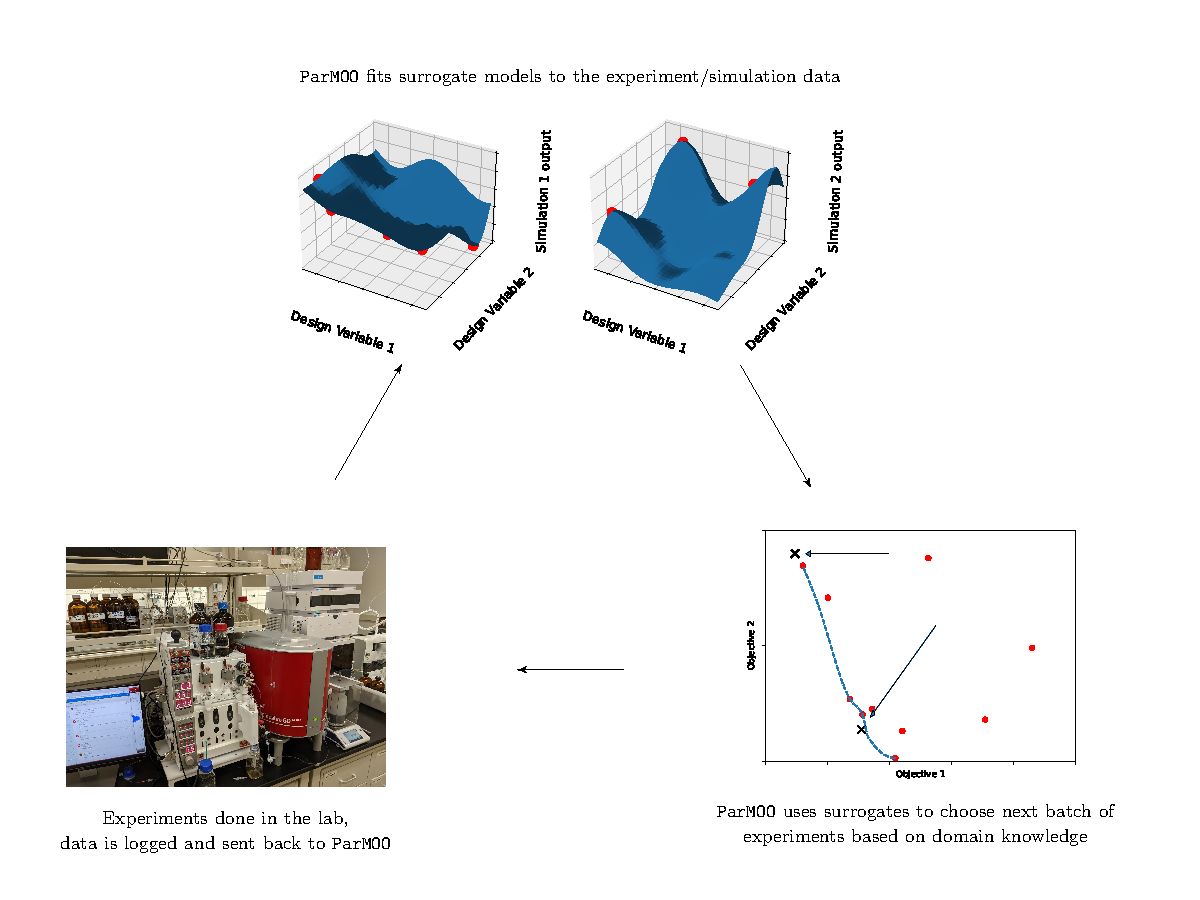
\includegraphics[width=0.75\textwidth]{../../img/moo_new/active-learning-loop.pdf}
  \end{center}
\end{frame}

%%%%%%%%%%%%%%%%%%%%%%%%%%%%%%%%%%%%%%%%%%%%%%%%%%%%%%%%%%%%%%%%%%%%%%%%%%%%%%
\begin{frame}
\frametitle{Our framework and software stack}
%%%%%%%%%%%%%%%%%%%%%%%%%%%%%%%%%%%%%%%%%%%%%%%%%%%%%%%%%%%%%%%%%%%%%%%%%%%%%%
  \begin{itemize}
  \item MDML gives us access to {\sl heterogeneous data from laboratory sources}
  \item ParMOO gives us modular/customizable {\sl modeling, embedding, and solvers}
  \end{itemize}

  \begin{center}

  \vskip -20pt

  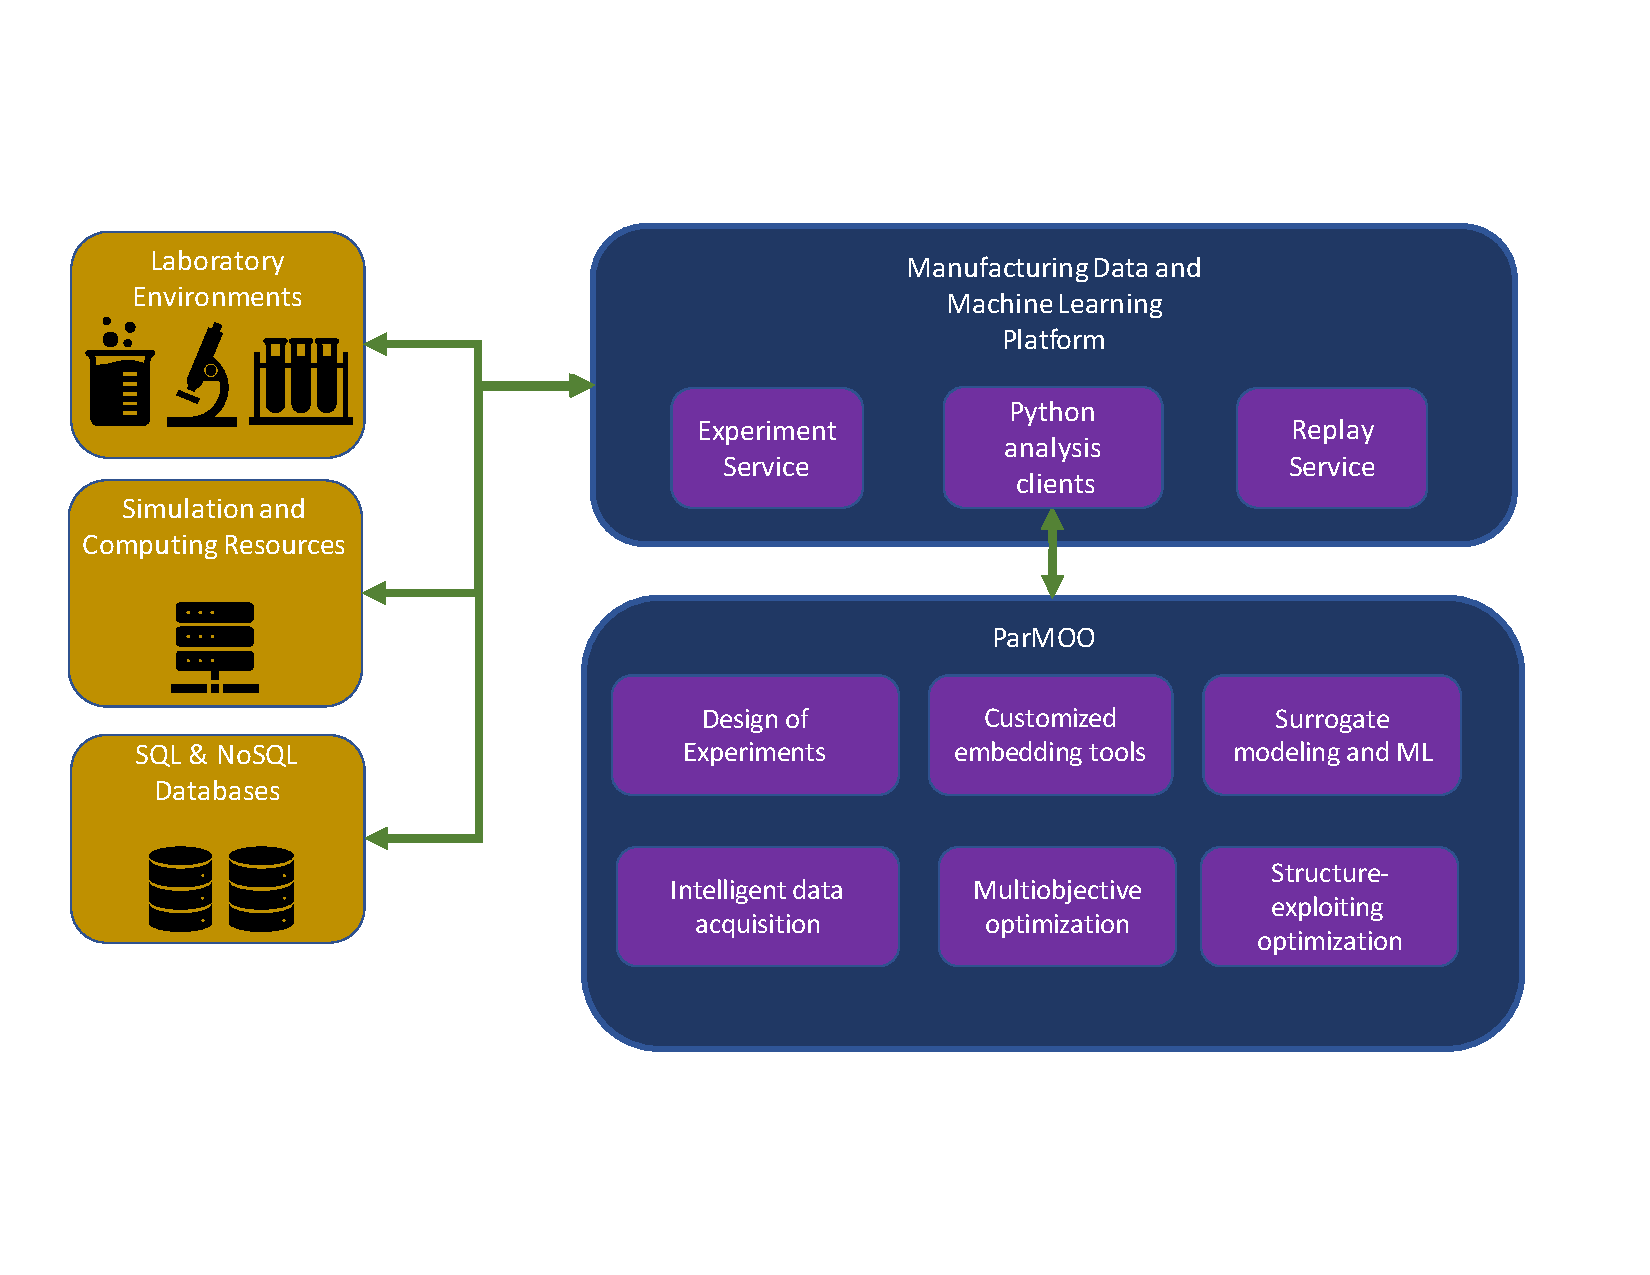
\includegraphics[width=0.75\textwidth]{../../img/moo_new/mdml-parmoo-2.pdf}\\
  Build \& deploy custom solvers for computational and experimental problem!
  \end{center}
\end{frame}

%%%%%%%%%%%%%%%%%%%%%%%%%%%%%%%%%%%%%%%%%%%%%%%%%%%%%%%%%%%%%%%%%%%%%%%%%%%%%%
\begin{frame}
\frametitle{Example: TFMC Manufacturing Conditions}
%%%%%%%%%%%%%%%%%%%%%%%%%%%%%%%%%%%%%%%%%%%%%%%%%%%%%%%%%%%%%%%%%%%%%%%%%%%%%%

  \begin{center}

  Optimize the production of TFMC via a known reaction...\\
  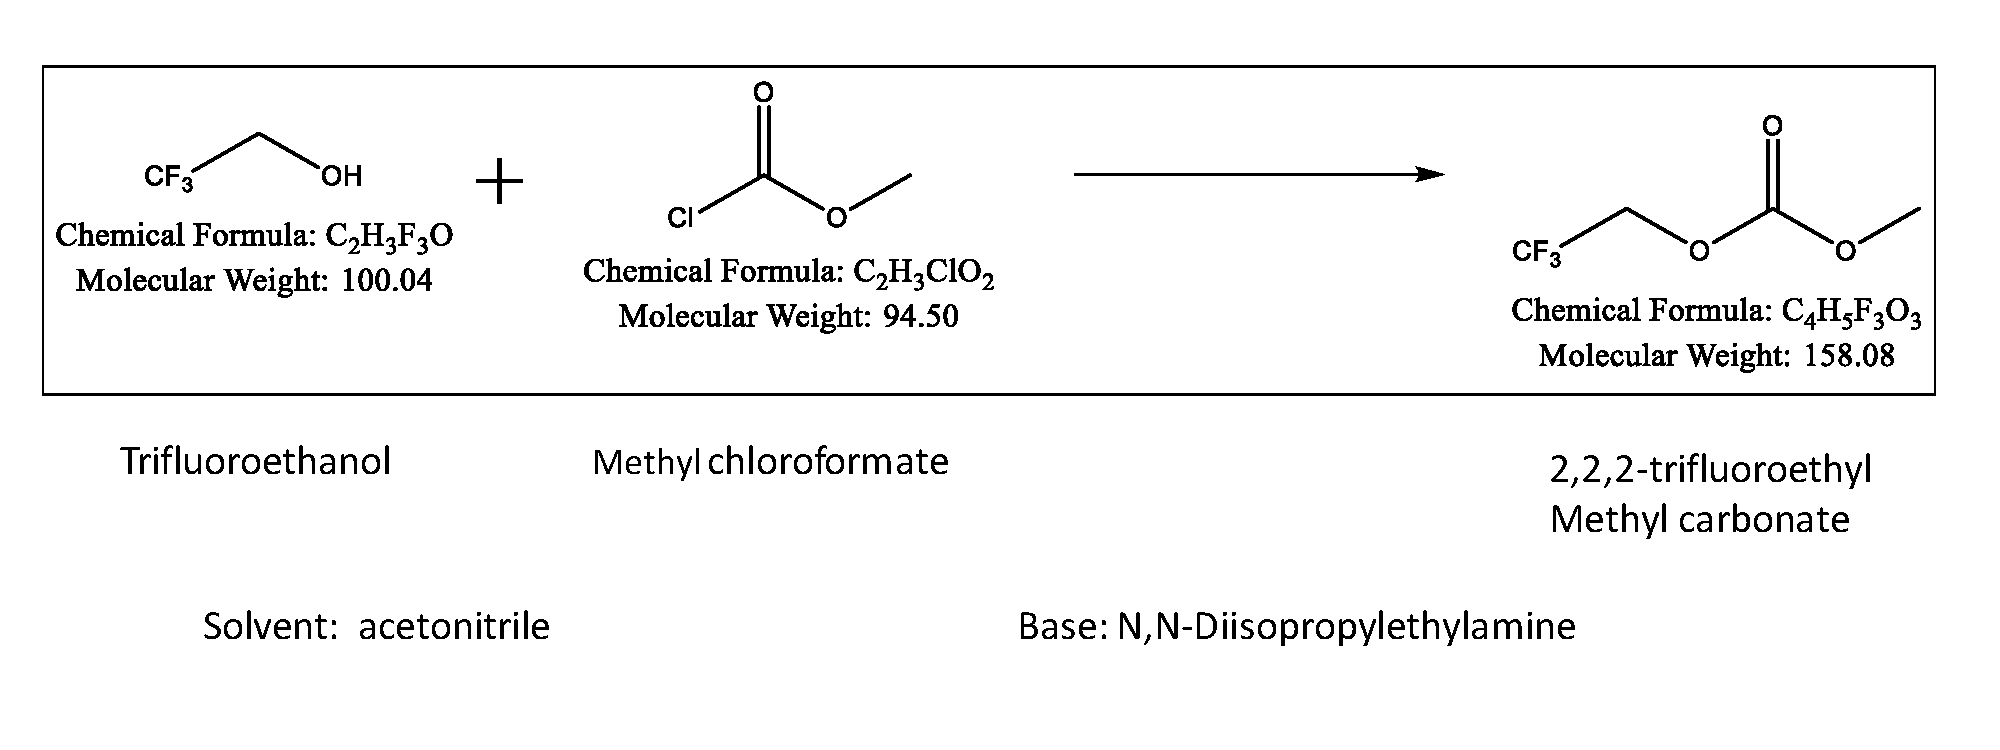
\includegraphics[width=0.75\textwidth]{../../img/probs/basic_reaction.pdf}\\
  \hbox{
   \hskip -90pt
    \vbox{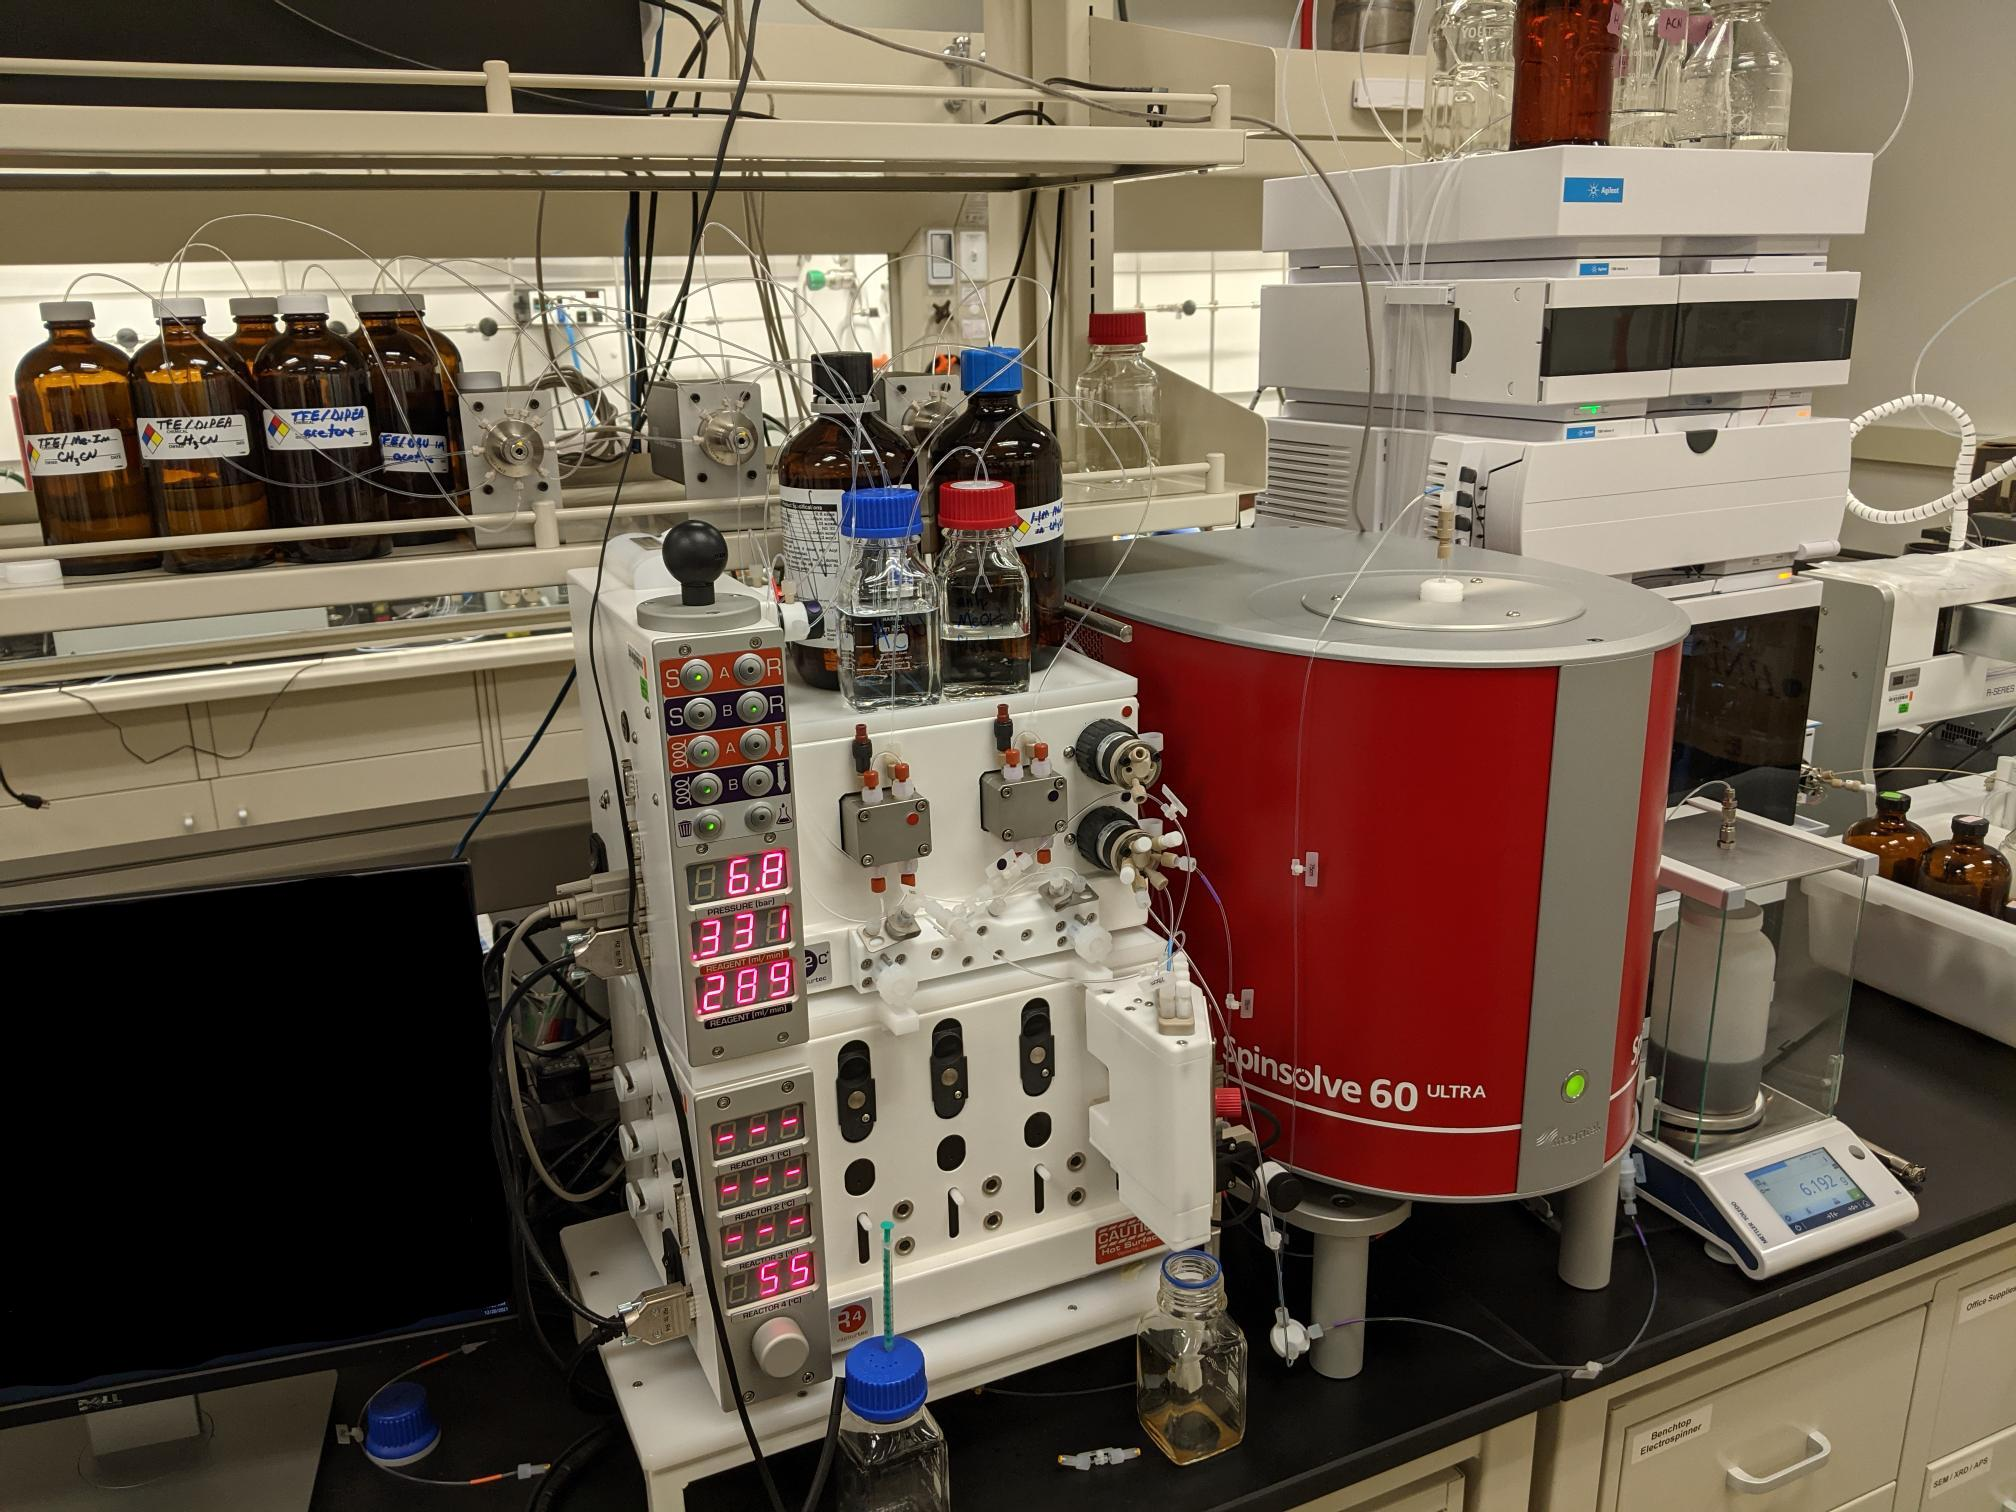
\includegraphics[width=0.31\textwidth]{../../img/probs/cfr-nmr-setup.jpg}}
    \hskip -190pt
   \vbox{... in LabVIEW automated CFR\\
    $\quad$ and measured via NMR\\
    $\quad$\\
    Left to right:\\
    PC running LabVIEW\\
    CFR and feed\\
    NMR spectroscope\\}
    }
  \end{center}
\end{frame}

%%%%%%%%%%%%%%%%%%%%%%%%%%%%%%%%%%%%%%%%%%%%%%%%%%%%%%%%%%%%%%%%%%%%%%%%%%%%%%
\begin{frame}
\frametitle{Problem definition}
%%%%%%%%%%%%%%%%%%%%%%%%%%%%%%%%%%%%%%%%%%%%%%%%%%%%%%%%%%%%%%%%%%%%%%%%%%%%%%
  \begin{itemize}
  \item {\bf Want to maximize TFMC production at high temperatures}
  \item High temperatures trigger a side-reaction and produces byproduct (TFE)
  \begin{itemize}
    \item {\bf Minimize TFE production}
  \end{itemize}
  \end{itemize}

  \bigskip

  {\sl Design variables and bound constraints for experiment:}

  \begin{center}
  \begin{tabular}{c|cc}
      Parameter & Lower bound & Upper bound \\
      \hline
       Temperature (degrees C) & 40 & 150 \\
       Reaction time (seconds) & 60 & 300 \\
       Equivalence ratio (no units) & 0.9 & 2 \\
  \end{tabular}
  \end{center}
\end{frame}

%%%%%%%%%%%%%%%%%%%%%%%%%%%%%%%%%%%%%%%%%%%%%%%%%%%%%%%%%%%%%%%%%%%%%%%%%%%%%%
\begin{frame}
\frametitle{Challenges and Solver Settings}
%%%%%%%%%%%%%%%%%%%%%%%%%%%%%%%%%%%%%%%%%%%%%%%%%%%%%%%%%%%%%%%%%%%%%%%%%%%%%%
  Solve a small problem on an extremely limited budget:
  \begin{itemize}
  \item 3 variable, 2 objective problem
  \item Experiments take about 10 mins and we have limited supply of reagent materials
  \item About 50 experiments max
  \end{itemize}

  \medskip

  Solver settings:
  \begin{itemize}
  \item 15-pt Latin hypercube, Gaussian RBF surrogate, L-BFGS-B optimizer
  \item 3 scalarizations per batch, sorted by temp (to speedup reaction)
  \item evaluated batch on CFR, TFMC and TFE peaks recorded by NMR
  \end{itemize}
\end{frame}

%%%%%%%%%%%%%%%%%%%%%%%%%%%%%%%%%%%%%%%%%%%%%%%%%%%%%%%%%%%%%%%%%%%%%%%%%%%%%%
\begin{frame}
\frametitle{Experiment Results}
%%%%%%%%%%%%%%%%%%%%%%%%%%%%%%%%%%%%%%%%%%%%%%%%%%%%%%%%%%%%%%%%%%%%%%%%%%%%%%
  \begin{center}
  {\sl Results after 41 experiments steered by our solver}\\
  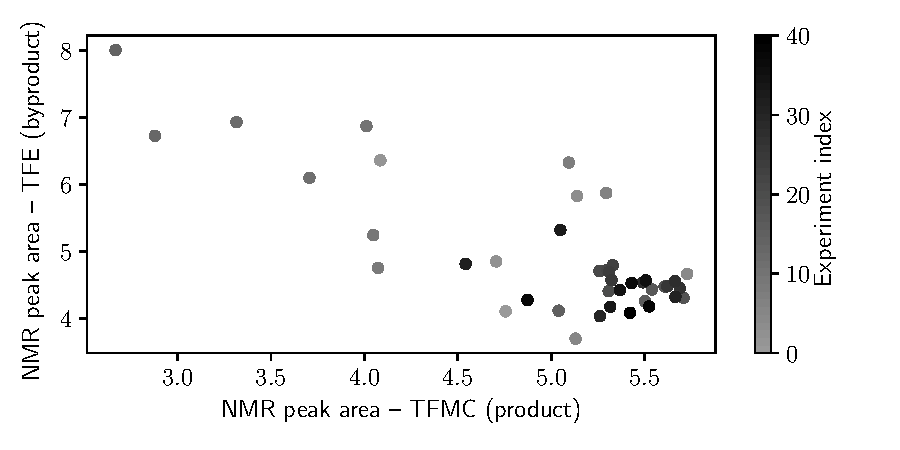
\includegraphics[width=0.7\textwidth]{../../img/moo_new/tfmc-tradeoff-eps-converted-to.pdf}\\
  \end{center}
\end{frame}

%%%%%%%%%%%%%%%%%%%%%%%%%%%%%%%%%%%%%%%%%%%%%%%%%%%%%%%%%%%%%%%%%%%%%%%%%%%%%%
\begin{frame}
\frametitle{Next Steps}
%%%%%%%%%%%%%%%%%%%%%%%%%%%%%%%%%%%%%%%%%%%%%%%%%%%%%%%%%%%%%%%%%%%%%%%%%%%%%%

  Need to handle more complex design spaces:\\
  \hbox{
  \vbox{
  \begin{itemize}
    \item Custom embeddings (including generative AI)
    \item Trust-region descent / subspace iterations
  \end{itemize}
  }
  \hskip -150pt
  \vbox{
  \begin{itemize}
    \item Custom surrogate models
    \item Structure-exploiting optimizers
  \end{itemize}
  }}

  \medskip

  \hbox{
  \vbox{
  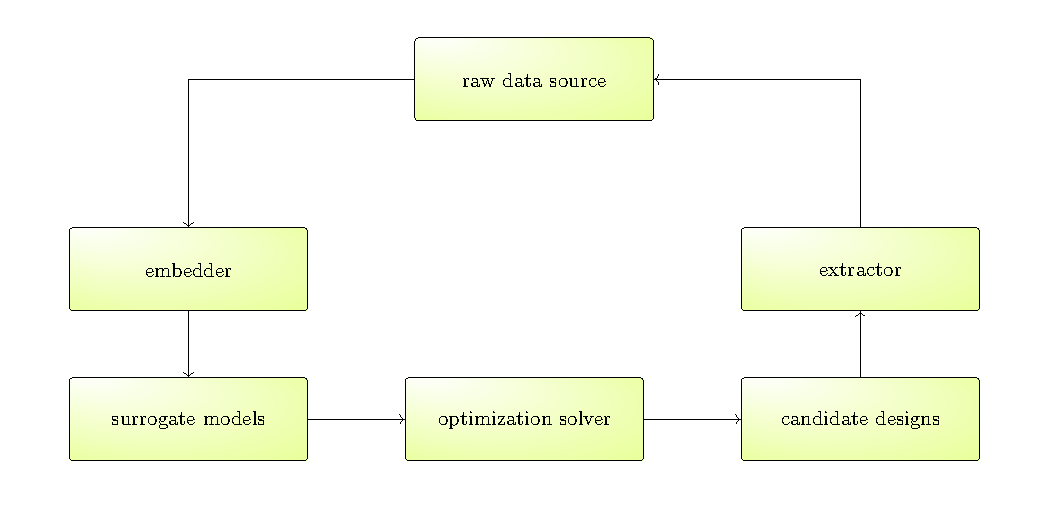
\includegraphics[width=0.55\textwidth]{../../img/moo_new/embedder-extractor.pdf}\\
  $\quad$\\
  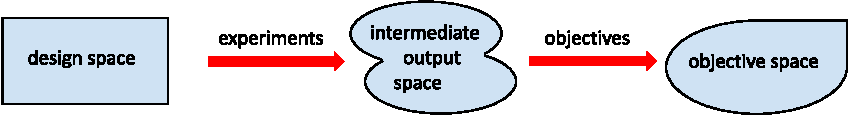
\includegraphics[width=0.6\textwidth]{../../img/moo_new/obj-sim-des-space-eps-converted-to.pdf}}
  \hskip -120pt
  \vbox{$\quad$\\
  (Top) using\\
  custom embedders\\
  to optimize in\\
  latent space\\
  $\quad$\\
  (Bottom) exploiting\\
  problem structure\\
  using composite\\
  objectives\\
  $\quad$\\
  $\quad$\\
  }}

\end{frame}

%%%%%%%%%%%%%%%%%%%%%%%%%%%%%%%%%%%%%%%%%%%%%%%%%%%%%%%%%%%%%%%%%%%%%%%%%%%%%%
\begin{frame}
\frametitle{A sneak peek!}
%%%%%%%%%%%%%%%%%%%%%%%%%%%%%%%%%%%%%%%%%%%%%%%%%%%%%%%%%%%%%%%%%%%%%%%%%%%%%%

  We created a surrogate problem based on this data to explore next steps!

  \medskip

  {\tt https://github.com/parmoo/parmoo-solver-farm}\\
  $\quad\rightarrow$ {\tt cfr-material-design-2022}\\

  \medskip

  \begin{center}
  5 variable (2 categorical), 3 objectives (1 cheap) problem\\
  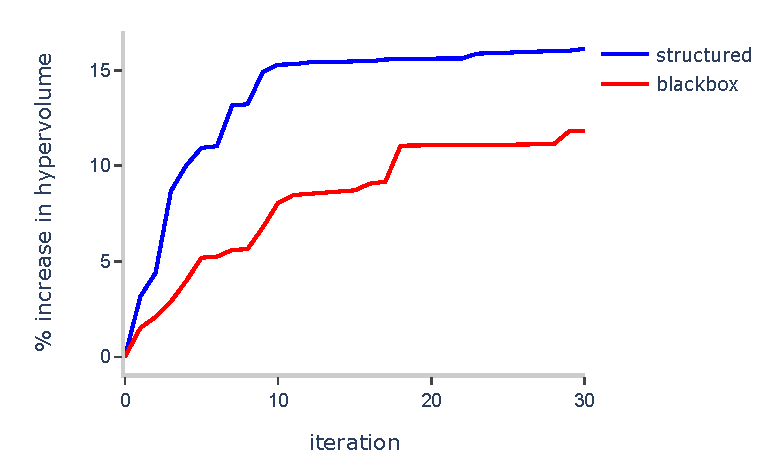
\includegraphics[width=0.7\textwidth]{../../img/probs/cfr-new-hypervol.pdf}
  \end{center}

  \medskip

  {\tt arxiv.org/abs/2304.06881}
  
\end{frame}

%%%%%%%%%%%%%%%%%%%%%%%%%%%%%%%%%%%%%%%%%%%%%%%%%%%%%%%%%%%%%%%%%%%%%%%%%%%%%%
\begin{frame}[plain]
%%%%%%%%%%%%%%%%%%%%%%%%%%%%%%%%%%%%%%%%%%%%%%%%%%%%%%%%%%%%%%%%%%%%%%%%%%%%%%

  \begin{center}
  Email: {\tt tchang@anl.gov}\\

  \bigskip

  {\color{red} We love open source!}\\

  {\tt git clone https://github.com/parmoo/cfr-materials\\
  pip install REQUIREMENTS.txt}

  \bigskip

  {\small

    This material was based upon work supported by the U.S.\ Department of
    Energy, Office of Science, Office of Advanced Scientific Computing
    Research, Applied Mathematics and SciDAC programs under Contract Nos.\
    DE-AC02-05CH11231 and DE-AC02-06CH11357 
    and by the Argonne LDRD program.     

  }
  \end{center}
\end{frame}
\end{document}
